\documentclass{thesis-ekf}
\usepackage[T1]{fontenc}
\PassOptionsToPackage{defaults=hu-min}{magyar.ldf}
\usepackage[magyar]{babel}
\usepackage{mathtools,amssymb,amsthm,pdfpages}
\usepackage{listingsutf8,xcolor,caption}
\definecolor{monokaiblue}{RGB}{102,217,239}
\definecolor{monokaicomment}{RGB}{117,113,94}
\definecolor{monokaired}{RGB}{249,38,114}
\definecolor{monokaigreen}{RGB}{166,226,46}
\definecolor{monokaipurple}{RGB}{174,129,255}
\definecolor{monokaiyellow}{RGB}{230,219,116}
\definecolor{bgcolor}{RGB}{39,40,34}
\renewcommand{\lstlistingname}{kód}
\lstdefinestyle{kod1}{
	inputencoding=utf8/latin2,
	language=PHP,
	basicstyle=\footnotesize\color{white}\mdseries,
	numbers=left,
	numberstyle=\color{black}\mdseries,
	xleftmargin=2cm,
	xrightmargin=2cm,
	breaklines,
	postbreak=\hbox{$\color{monokaiyellow}\hookrightarrow\ $},
	backgroundcolor=\color{bgcolor},
	frame=tblr,
	framesep=3pt,
	keywordstyle=\sffamily\mdseries,
	commentstyle=\it\color{monokaicomment},
	keywords=[1]{function,session_unset,session_destroy,header,array_key_exists,is_numeric,sha1,getRecord,empty,executeDML},
	keywordstyle=[1]\color{monokaiblue}\textbf,
	keywords=[2]{require_once,if,return},
	keywordstyle=[2]\color{monokaired}\textbf,
	keywords=[3]{IsUserLoggedIn,UserLogout,UserLogin,UserRegister},
	keywordstyle=[3]\color{monokaigreen}\textbf,
	keywords=[4]{null,false,DATABASE_CONTROLLER},
	keywordstyle=[4]\color{monokaipurple}\textbf,
}
\lstset{showstringspaces=false}
\DeclareMathOperator{\arctg}{arctg}
\footnotestyle{rule=fourth}
\theoremstyle{definition}
\newtheorem{definicio}{Definíció}[chapter]

\begin{document}
\institute{Matematikai és Informatikai Intézet}
\title{Beadandó feladat}
\author{Krigovszki Bálint\\Programtervező Informatikus BSc.}
\supervisor{Dr. Tómács Tibor\\egyetemi docens}
\city{Eger}
\date{2022}
\maketitle
\tableofcontents

\chapter*{Bevezetés}
\addcontentsline{toc}{chapter}{Bevezetés}
Ezen a helyen az örökös sötétség uralkodik. Nincs nap, nincs hajnal, csak az éjszaka állandó
feketesége. Fény nem származik máshonnan, csak az ezerfelé ágazó villámokból, amelyek
szeszélyesen cikáznak a haragos felhők között. A nyomukban vad dörgések rázzák meg az
égboltot, és sűrű, fagyos záporokat szabadítanak el. A vihar közeleg, és nincs menekvés\dots

Revan szeme felpattant, a rémálmában átélt rettegés immáron a harmadik éjszakán verte fel álmából.

Csendesen, mozdulatlanul feküdt, a bensőjére összpontosított, és hogy megnyugtassa
hevesen dübörgő szívét, a Jedi-törvények első sorát ismételgette magában: ,,Nincsenek
érzések, csak a lelki béke létezik\dots''
\cite{Jeffrey}

Még most is, két évvel azután, hogy visszanyerte az eredeti személyiségét, nehezen
békítette össze a tükörben látott arcot azzal a férfival, aki ő volt, mielőtt a Jedi Tanács
visszatérítette a világos oldalra.

Revan: a Jedi, a hős, az áruló, a hódító, a gonosztevő, a megmentő. Ő volt mindez, de ennél
több is: eleven legenda, a mítosz és a folklór megtestesítője, örök hírű történelmi személyiség.
Es mégis, a tükörből egy teljesen hétköznapi férfi nézett vissza rá, aki már a harmadik éjszakát
töltötte ébren.

\chapter{Dromund Kaas}
\section{Kaas City}
Mialatt kiszállt a kompból, Scourge Nagyúr a fejére húzta köpenyének csuklyáját, hogy óvja
arcát a széltől és záportól. Itt, a Dromund Kaason a viharok gyakorlatilag egymást érték. Sötét
felhők takarták el a napot örökkön-örökké, értelmetlenné változtatva a nappal és az éjszaka
kifejezéseket. Természetes világosság nem származott máshonnan, csak az égen átívelő,
gyakori villámokból, viszont az űrkikötő és a közeli Kaas City lámpái elég fényt szolgáltattak
ahhoz, hogy a Nagyúr lássa, hová lép.

Az erős elektromos viharok voltak a fizikai megnyilvánulásai a sötét oldal energiáinak,
amelyek áthatották az egész bolygót. Ezek vonzották ide a Sitheket ezer esztendővel ezelőtt,
amikor a puszta fennmaradásuk is kétségesnek tűnt.

A Nagy Hipertéri Háborúban elszenvedett, megsemmisítő vereség után a Császár\footnote{Tenebrae, a Sith Birodalom Császára.}, aki
valamivel korábban emelkedett fel a megmaradt Sithek megtépázott soraiból, elvezette
megfogyatkozott híveit ide, a Galaxis mindentől távol eső zugába. A köztársasági seregek és a
bosszúszomjas Jedik elől menekülve végül a köztársaságiak által feltérképezett űr határain túl,
az ősi szülőbolygójukon telepedtek le.



\begin{figure}[!ht]
	\centering
	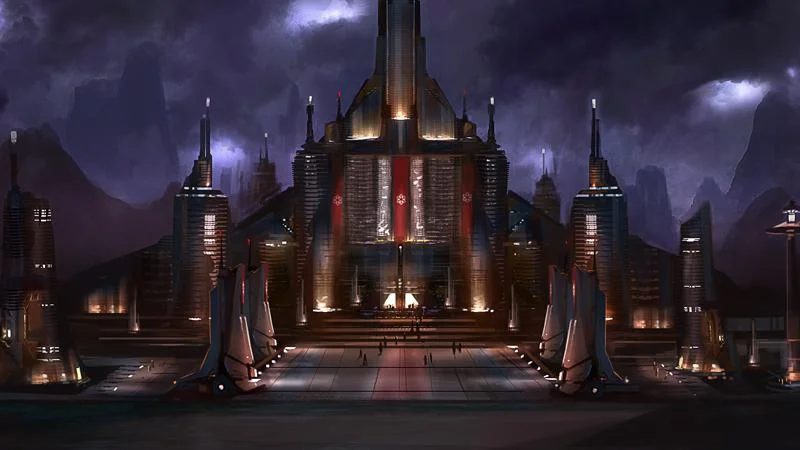
\includegraphics[width=5cm]{kaascity}
	\caption{Kaas City}
	\label{figure-kaascity}
\end{figure}

Itt, biztonságosan elrejtőzve az ellenségeik elől, a Sithek elkezdték újjáépíteni a Birodalmukat.
A Császár irányította őket, a halhatatlan és szörnyű hatalmú megmentő, aki ezer éve uralkodott
felettük. Az ő bölcs vezérletével felhagytak a barbár ősök élvhajhász életstílusával, és
megteremtettek egy majdnem tökéletes társadalmat, amelyben a birodalmi katonaság
működtette és ellenőrizte a mindennapi élet gyakorlatilag valamennyi mozzanatát. Gazdálkodók,
gépészek, tanárok, szakácsok és takarítók -- mindannyian részei lettek egy gigászi katonai
gépezetnek, amelynek valamennyi apró alkatrészét alaposan kiképezték, hogy a lehető
legnagyobb fegyelmezettséggel és hatékonysággal végezze a feladatait. Ennek eredményeként
a Sithek egyik világot a másik után hódították meg a Galaxis felfedezetlen régióiban, mígnem a
hatalmuk és befolyásuk utolérte, majd túlszárnyalta azt, amit a múltban élveztek.

Újabb villám lobbant az égen, egy pillanatra megvilágítva a Kaas City fölé magasodó
fellegvárat. A rabszolgák és odaadó hívek által emelt építmény egyszerre szolgált palotaként,
bevehetetlen erődként, valamint találkozóhelyként, ahol az uralkodó összeülhetett a Sötét
Tanácsot\footnote{A Sith Birodalom vezető szerve.} alkotó tizenkét válogatott Sith Nagyúrral és Úrnővel.
\cite[66.~oldal]{Jeffrey,Paul}

\section{Scourge Nagyúr}
Egy évtizeddel korábban, amikor Scourge első ízben, még ifjú tanítványként megérkezett a
Dromund Kaasra, megesküdött, hogy egy szép napon sétál egyet a citadella fényűző, zárt
termeiben. És mégis, noha éveket töltött a város határában működő Akadémián, Sosem
részesült ebben a kiváltságban. A legjobb tanítványok közé tartozott, az elöljárói hamar
felfigyeltek rá, mert mélyen áthatotta az Erő, és mert valósággal égett a tudásvágytól. Ám
tanítványok nem nyertek bebocsátást a fellegvárba, annak titkait azoknak tartogatták, akik
közvetlenül a Császárt és a Sötét Tanácsot szolgálták.

A sötét energiák hihetetlen erővel áradtak az építményből. Scourge az Akadémián töltött évei
alatt mindvégig érzékelte a heves, sistergő erőket. Merített belőlük, majd a tudatával és a
lelkével egyaránt összpontosítva átcsatornázta őket a testén, hogy életben maradjon a
kegyetlen felkészülés alatt\dots

És most, majdnem kétévnyi távollét után Visszatért a Dromund Kaasra. A leszállópályán állva
ismét megérezte a sötét oldalt a csontjaiban, azt a bizsergető izzást, amely bőségesen
kárpótolta a szél és az eső miatti kellemetlenségekért. De most már nem egyszerű
tanítványként érkezett ide, a Birodalom központjába, hanem teljes jogú Sith Nagyúrként.

Mindig is tudta, hogy egyszer eljön ez a nap. Annak idején remélte, hogy az Akadémia
elvégzése után a Dromund Kaason fog állomásozni. Ezzel szemben elküldték a Birodalom
határvidékére, hogy segítsen eltaposni néhány kisebb lázadást az újonnan meghódított
bolygókon. Gyanította, hogy a felettesei valamilyen fajta büntetésnek szánták ezt a
megbízatást. Valószínűleg az egyik instruktora, aki irigyelte az ő képességeit, azt javasolta,
hogy helyezzék a lehető legmesszebbre a Birodalom hatalmi központjától, hogy minél
lassabban fejlődjön, és haladjon felfelé a ranglétrán.

A rosszakarói balszerencséjére Scourge nem igazolta az elméletet. Noha száműzték a
Birodalom külső határainak civilizálatlan szektoraiba, sikerült jelentős hírnevet szereznie. A harci
jártassága révén, és mert könyörtelenül hajszolta a lázadók vezéreit, felhívta magára néhány
kiváló katonai vezér figyelmét. Most pedig, két évvel azután, hogy elhagyta az Akadémiát,
újonnan felkent Sith Nagyúrként tért vissza a Dromund Kaasra. Ami ennél is fontosabb, Darth
Nyriss hívta ide személyesen, a Sötét Tanács legrégebbi tagjainak egyike.

-- Scourge Nagyúr! -- kiáltotta egy futva közeledő alak. -- Sechel vagyok! Üdvözlöm a
Dromund Kaason! Örülök, hogy megérkezett!

-- Hogy visszatért\dots -- javította ki mogorván Scourge a férfit, aki időközben fél térdre
ereszkedett előtte, és tisztelete jeléül fejet hajtott. -- Nem most járok itt először.

Hozzá hasonlóan Sechel is viselte a csuklyáját, hogy védekezzen az eső ellen, de mialatt
közeledett, Scourge meglátta a fickó vörös bőrét, illetve az álláról lecsüngő nyúlványokat. A
beszédes jelekből tudta, hogy az idegen hozzá hasonlóan tiszta vérű Sith, de vele ellentétben
alacsony, vézna nyomorult volt. A tudatát kiterjesztve érzékelte, hogy éppen csak pislákol
benne az Erő, és a felismerés nyomán undorodva fintorgott.

A Birodalom lakosságának zömét alkotó emberektől eltérően a Sith-fajok, ha különböző
mértékben is, de érzékelték az Erőt. Ez különböztette meg őket, ezért váltak a rendszer
elitjévé, ez emelte ki őket a társadalom alsó rétegeiből. És ez volt az az örökség, amit
elszántan védelmeztek.

Egy tiszta vérű személy, akit nem fűztek kapcsolatok az Erőhöz, maga volt a förtelem. A
szokások szerint egy efféle teremtmény nem érdemelte meg az életet. Az Akadémián töltött
évek alatt Scourge Nagyúr találkozott néhány Sithtel, akiket feltűnően csekély mértékben hatott
át az Erő. Különleges képességek híján magas rangú családjaik befolyására támaszkodva
szereztek maguknak állást az Akadémián, mint alacsonyabb szintű szárnysegédek vagy
hivatalnokok, vagyis olyan helyeken szolgáltak, ahol a fogyatékosságuk kevésbé tűnt fel.
Ezeket az alakokat csakis a tiszta vérű származásuk mentette meg az alsó kasztoktól, és
Scourge szemében alig voltak jobbak a rabszolgáknál, bár azt el kellett ismernie, hogy a
tehetségesebbek néha hasznosnak bizonyultak.\cite{John}

De még sosem találkozott a saját fajtájából olyannal, akit olyan gyenge szálak fűztek az
Erőhöz, mint azt a férfit, aki most a lába előtt térdelt. Nyugtalanítónak találta a tényt, hogy
Darth Nyriss egy ilyen hitvány senkit küldött elé. Sokkal látványosabb, sokkal lenyűgözőbb
fogadtatásra számított.
\section{A merénylet}
Tágas udvarban landoltak, amelyet északról és délről magas kőfalak határoltak. A keleti oldal
nyitott volt az utca felé, a nyugatit Darth Nyriss erődjének homlokzata zárta le. Az építmény
számos vonásában a Császár palotájára emlékeztetett, bár természetesen jóval kisebb volt
annál. Az építészeti hasonlóságok nem csupán az uralkodó iránti tiszteletadásról szóltak. Akár
az ő fellegvára, úgy ez az épület is egyszerre szolgált Nyrissnek lakóhelyként és erődként, ahol
baj esetén meghúzhatta magát. Úgy tervezték és építették, hogy egyszerre legyen díszes,
lenyűgöző és könnyen védhető.

Magát az udvart féltucatnyi szobor díszítette. A talapzatuk szélessége elérte a három métert,
a magasságuk az ötöt is meghaladta. A két legnagyobb a Sithek hagyományos köpenyét
viselő, humanoid teremtményeket örökítette meg, egy férfit és egy nőt. A karjukat kissé maguk
elé emelve, a tenyerüket felfelé fordítva álltak. A férfi arcát csuklya rejtette -- szerte az egész
Birodalomban így szokták ábrázolni a Császárt. A nő hátravetve viselte csuklyáját, hogy
felfedje harcias vonásait. Scourge tudta, hogy ha a szobrász pontosan dolgozott, akkor ő ezt az
arcot fogja látni, amikor első ízben megpillantja Darth Nyrisst.

A többi szobor absztrakt alkotás volt, de mindegyik magába foglalta Nyriss címerét, a tágas
körbe zárt, négyágú csillagot. A talajt finom, fehér kavics borította. Körös-körül díszítő
alakzatokat lehetett látni rajta, amelyeket egy más világokon nem létező, ritka zuzmóból
alakítottak ki. Ez a növény különös módon élt és virult a Dromund Kaas örökös sötétjében, és
halvány, lila fényt bocsátott ki, amely kísérteties derengésbe vonta az egész udvart. A
kisméretű leszállópályától kiindulva keskeny, kövezett járda vezetett egészen az erőd
főbejáratáig.

Sechel kiugrott a járműből, gyorsan megkerülte, és kinyitotta az ajtót az előkelő utasnak.
Scourge kilépett a siklóból a jéghideg esőbe, amely ugyanolyan sűrűn zuhogott itt, mint a város
másik oldalán.

-- Erre parancsolj, Nagyuram! -- hadarta Sechel, és elindult az épület felé.

Scourge a szolga nyomába szegődött, és mialatt átvágott az udvaron, mindvégig arra
számított, hogy közeledtére a bejárat kinyílik. Aztán meglepetten tapasztalta, hogy a
kétszárnyú kapu zárva maradt. Sechel nem hökkent meg, az ajtó mellé épített holokészülékhez
lépett, és megnyomta a hívógombot.

A tenyérnyi lemez felett kéken villódzó fényalak jelent meg, egy körülbelül negyvenéves férfi
háromdimenziós képmása. Az illető egyszerű, de elegáns egyenruhát viselt, melynek láttán
Scourge megsejtette, hogy a férfi Nyriss személyi testőrségének parancsnoka.

-- A vendégünk megérkezett, Murtog! -- jelentette Sechel a Nagyúr felé biccentve.

-- Ellenőrizted a személyazonosságát? -- érdeklődött a Murtognak nevezett tiszt.

-- Te\dots te meg miről beszélsz? -- hebegte ijedten Sechel.

-- Honnan tudhatnánk, hogy ő az igazi Scourge Nagyúr?

A kérdés szemmel láthatóan teljesen megdöbbentette a szolgát.

-- Én nem\dots úgy értem\dots úgy tűnik\dots szóval\dots

-- Nem engedem be, amíg nem kapok bizonyítékot -- jelentette ki Murtog.

Sechel a válla felett visszanézett a Nagyúrra, az arcáról lerítt, hogy megalázva érzi magát, és
hogy retteg. Aztán közelebb hajolt a holokészülékhez, és fojtott hangon folytatta:

-- Ez teljesen felesleges. Túlléped a hatáskörödet!

-- Én vagyok a biztonsági főnök -- emlékeztette őt Murtog. -- Éppen ezért bőven belül van a
hatáskörömön. Adj öt percet, amíg ellenőrzöm, hogy minden rendben van-e.

Scourge lépett egyet előre, vállon ragadta, és oldalra lökte Sechelt, majd haragosan
ráförmedt a fényalakra:

-- Hogy merészelsz megsérteni azzal, hogy idekint várakoztatsz az esőben, mint valami
koldust? Vendég vagyok! Maga Darth Nyriss hívott ide!

Murtog kurta gúnykacajt hallatott.

-- Ez a kijelentés talán nem pontosan fedi a valóságot -- válaszolta vigyorogva, azzal
megszakította az adást.

Scourge megfordult, és meglátta Sechelt, aki tőle nem messze, reszketve lapult a falhoz.

-- Sajnálom, Nagyuram! -- mondta rekedtes hangon. -- Murtog eléggé paranoiás lett,
amióta\dots

-- Hogy értette azt, hogy nem fedi a valóságot? -- vágott közbe Scourge. -- Darth Nyriss
hívott ide, vagy nem?

-- Igen. Hát persze, hogy ő\dots bizonyos értelemben\dots

Scourge a férfi felé nyújtotta a kezét, és megidézte magában az
Erőt. A szolga mindkét kezével a torkához kapott, és fuldokolni kezdett, közben a levegőbe
emelkedett, mintha egy láthatatlan kéz ragadta volna meg.

-- Most pedig elmondod, hogy mi folyik itt -- mondta Scourge tökéletesen érzelemmentes
hangon. -- Mindent elmondasz, vagy meghalsz. Megértetted?

Sechel megpróbált beszélni, de csak krákogni és hörögni tudott, így aztán kétségbeesetten
bólogatott. Scourge beérte ennyivel, és elengedte. Sechel hirtelen egy teljes méternyit zuhant,
majd elterült a kövezeten, és fájdalmában hangosan nyögdécselve feltérdelt.

-- Nem Darth Nyriss ötlete volt, hogy idehívjon téged -- magyarázta a fuldoklástól reszelős
hangon. -- A második orgyilkos merényletet követően a Császár felvetette, hogy talán az Úrnő
háznépéből is érintett valaki. Azt javasolta neki, hogy vonjon be egy kívülállót.

Hirtelen minden értelmet nyert. Az uralkodó akarata előtt mindenki meghajolt. A ,,javaslatát''
gyakorlatilag parancsnak kellett venni. Scourge most már tudta, hogy Nyriss azért hívta őt ide,
mert nem volt más választása. Mindeddig azt hitte, hogy díszvendégként fogják kezelni, de
valójában nem számíthatott másra, mint hogy betolakodónak tekintik. A puszta jelenléte
sértette az Úrnő hűséges híveit, és mindenkit arra emlékeztetett, hogy a Császár nézete szerint
Nyriss nem képes egyedül elbánni az orgyilkosokkal. Ezek után nem csodálkozott azon, hogy
olyan szegényes fogadtatásban részesült, sem pedig azon, hogy Nyriss testőrségének
parancsnoka annyira ellenségesen bánt vele.

Scourge rájött, hogy rendkívül kényes helyzetbe került. Joggal számíthatott arra, hogy a
merényletsorozat kitervelői után folytatott nyomozása alatt mindenhol ellenállásba és
gyanakvásba fog ütközni. Minden hibát, még azokat is, amelyeket nem követ el, őrá fognak
kenni. Egyetlen rossz lépés véget vethet a pályafutásának vagy akár az életének is.

Még akkor is ezeket az új felismeréseit emésztette, amikor meghallotta, hogy egy sikló
közeledik felé a vihartól dúlt égbolton. A teljesen hétköznapi hang ártalmatlannak tűnt, de az
érzékei valamiért riadófokozatba kapcsoltak. A szíve hevesen vert, a légzése felgyorsult. A
vérébe tóduló adrenalintól az állnyúlványai rángatóztak, az izmai megfeszültek.

Kezébe vette a fénykardját, és felnézett az égre. A lába előtt görnyedező Sechel felkiáltott,
és eltakarta fejét a kezével, mert azt hitte, a Nagyúr neki szánja az energiapengét. Scourge
azonban nem törődött a hitvány alakkal.

A vihar miatti sötétségben éppen csak meglátta a sikló körvonalait, de azt meg tudta állapítani, hogy egyenesen felé tart. Az erőn keresztül megszondázta a járművet és az utasait. Nyomban feltámadt benne a harag, mert a gyanúja beigazolódott: akárkik ültek abban a gépben, azért jöttek, hogy végezzenek vele.

Ez az egész, attól a pillanattól kezdve, hogy Scourge felfigyelt a siklóra, addig a pillanatig,
amíg meggyőződött az idegenek ellenséges szándékairól, kevesebb mint két másodpercet vett
igénybe. De ennyi idő is elég volt a támadóknak ahhoz, hogy megközelítsék, és lecsapjanak rá.

Sugárnyalábok száguldottak felé, mire ő gyorsan félreszökkent. A kavicsra érkezve gurult
egyet, majd azonnal felpattant, éppen idejében ahhoz, hogy kitérjen a második sorozat elől. Az
Erőtől kölcsönzött, szemkápráztató gyorsasággal átrohant az udvaron, közben minden
lépésénél lövedékek csapódtak a talajba, alig egy-másfél méterrel a háta mögött. Egy utolsó,
elnyújtott ugrással bevetődött a Császár szobra mögé, és gondolatban felmérte a helyzetet.

A sikló minden jel szerint automata célzórendszerrel felszerelt, sorozatlövő sugárvetőt
hordozott, máskülönben a lövések nem követhették volna ilyen pontosan. Márpedig egy effajta
fegyver elől még egy Sith Nagyúr sem térhetett ki az örökkévalóságig. Meg kellett bénítania a
járművet.

A sikló elkanyarodott tőle, majd jobb fordulót kezdett a következő rácsapáshoz. Mielőtt
azonban befejezte volna, Scourge kilépett a szobor mögül, és felhajította a fénykardját. A vörös
penge forogva száguldott a sötét égbolt felé, kezdetben tágas, de egyre szűkülő ív mentén.
Lenyírta a sikló farát, aztán a röppályáján végigrepülve visszatért Scourge felnyújtott kezébe.

A légi jármű hajtóművének búgása fejhangú visítássá változott. A tatjából sűrű, fekete füst tört
elő, amelyet éppen csak látni lehetett a sötét égbolttal a háttérben. A sikló dülöngélt és
bukdácsolt, gyors ütemben veszített magasságából, de az utasai ismét tüzet nyitottak.

Scourge visszaugrott a Császár szobra mögé, és szilárdan nekivetette hátát a talapzatnak,
közben újabb töltetek záporoztak rá. A következő másodpercben a sikló elhúzott felette,
immáron olyan alacsonyan, hogy gyakorlatilag lefejezte a műalkotást, amely mellett fedezéket
keresett.

A súlyos kődarab egyenesen felé zuhant, így félre kellett ugrania előle, máskülönben
agyonütötte volna. Ezzel egy időben meglátta, hogy a sikló a talajba vágódik. A vészhelyzeti
lebegtetőrendszer elnyelte az ütés erejét, és megmentette a járművet attól, hogy darabokra
zúzódjon, de a sérült hátsó hajtómű darabjai így is szerteszét repültek.

Scourge fénykardját a feje fölé lendítve rohant a lezuhant jármű felé. A roncsból két utas
kászálódott ki. A kényszerleszállás alaposan megrázta őket, de sértetlenek maradtak. A
Nagyúr éppen csak egy kicsit lepődött meg, amikor felismerte a vörös ruhás zsoldosokat,
akikkel az űrkikötő mellett találkozott.

\chapter{Coruscant}\label{fejezet-coruscant}
\section{Galaktikus Piac}
A coruscanti Galaktikus Piacon ugyanolyan sokan nyüzsögtek, mint mindig, de senki sem
vette észre Revant, mialatt átvágott a tömegen. Majdnem két év telt el azóta, hogy kikiáltották
a Galaxis megmentőjének. Jóllehet a Szenátus megadta neki a legmagasabb kitüntetést, a
Dicsőség Keresztjét, és az átadó ünnepségét élőben közvetítette az egész HoloHálózat,
továbbá sokan ismerték a nevét, hétköznapi és eléggé jellegtelen vonásai hamar eltűntek a
polgárok emlékezetéből. Az ünnepséget követőén visszavonult hős lett belőle. Tudatosan
kerülte a nyilvános fellépéseket, és mindenkit visszautasított, aki interjút kért tőle. Leborotválta
a szakállát, és ritkán viselte Jedi-köpenyét, aminek köszönhetően ritkán fordult elő, hogy
felismerték az utcán.

A névtelenség és ismeretlenség tökéletesen megfelelt neki. Többek között ezért telepedett le
a Coruscanton. A bolygót egymilliárd teremtmény lakta, és ő könnyűszerrel beleolvadt a
sokaságba. Ez még könnyebben ment itt, a Galaktikus Piacon, a Köztársaság központjának
legtarkább, legzavarosabb negyedében. Gyakorlatilag valamennyi ismert fej kereskedői és
boltosai gyűltek össze itt, hogy a legkülönfélébb színű, formájú és méretű árucikkek millióit
kínálják. Vörös bőrű togrutatiak vegyültek kék bőrű twi’lekkel, alacsony sullustiak alkudoztak
hatalmasról hízott huttokkal, halszerű mon calamarik osztották meg az utcákat ragadozó
macskákra emlékeztető catharokkal. Ebben a színes, zűrzavaros és érdekes sokaságban senki
sem szentelte a figyelmét egyetlen, magányos embernek és az ő asztrodroidjának.

Sajnálatos módon a figyelem hiánya azt is jelentette, hogy a Revan mögött guruló T3-M4-et
szinte minden pillanatban oldalba vágták, megrúgták vagy éppen átestek rajta. A droid sértett
és dühös dudálások és füttyök folyamatos áradatával fejezte ki a nemtetszését.

Néhány perccel később valóban megérkeztek az úti céljukhoz. A Dealer’s Den nevezetű,
kisebbfajta kocsma a Galaktikus Piac egyik eldugott részén működött, italokkal, táncosokkal és
szerencsejátékkal várta a vendégeit. Ezt a szórakozóhelyet főleg a coruscanti társadalom
csőcseléke látogatta: feketepiaci ügyeskedők, csempészek, rablók, fejvadászok és
drogkereskedők. Ennek eredményeként a vendégkör csupa gyanús alakból állt, elsősorban
rossz hírű fajok egyedeiből. Az asztalok körül főleg rodiaiak, chevinek és kubazok üldögéltek.
Alig maroknyi ember akadt a söntésben, köztük az a férfi, akit Revan keresett: Canderous
Ordo.

A mandalori magányosan ült az egyik sarokasztalnál, szokásához híven a hátát a falnak
vetve. A megszokott ruházatát viselte, homokszínű nadrágot és ujjatlan, fekete pólót, amely
szabadon hagyta vaskos izmokkal teli karját, és látni engedte a bal vállára tetovált kláncímert.
A fejét majdnem teljesen kopaszra borotválta, csak a tetején húzódott végig egy rövidre nyírt
sáv, és ez a hajviselet még jobban kihangsúlyozta erős, szögletes állkapcsát, valamint darabos,
erőszakos arcvonásait. Minden ízében szabadúszó zsoldosnak látszott, bár Revan tudta róla,
hogy nem vállalt munkát, mióta két évvel ezelőtt együttes erővel legyőzték Darth Malakot.
\section{Hallion}
A Hallion, ez a kicsi és jelentéktelen bolygó a Magtól\footnote{A Galaxis középpontja körül elhelyezkedő csillagrendszerek.} messze, a főbb hiperutaktól távol
keringett, tucatnyi másik világ között, amelyek szintén a Birodalom fennhatósága alá tartoztak.
Egyetlen említésre méltó vonása akadt, hogy hét apró, természetes égitest vette körül,
amelyek olyan kicsik voltak, hogy alig minősültek holdnak. Ezen az estén négy hold kitelve
ragyogott az égen, és együttes fényük elég világosságot adott ahhoz, hogy Scourge éjjellátó
készülék nélkül is tisztán lássa az Uxiol Droidgyár részleteit.

-- A tervrajzodon nyoma sincs védőkerítésnek -- suttogta ingerülten.
Ő és Sechel egy kisebbfajta, ritkás ligetben hasaltak egy mező szélén, körülbelül húsz
méterre a telep határától.

-- Talán nemrégiben építették -- felelte szintén fojtott hangon a tanácsadó. -- De nem lesz
vele gondunk. Ha átjutsz a másik oldalára, egyszerűen kinyitod nekem a kaput, és beengedsz.

Scourge már valamivel korábban felfigyelt arra, hogy Sechel jelentősen megváltozott a
küldetés alatt. Mintha kicserélték volna. Az alázatos talpnyaló, aki a Dromund Kaas
űrkikötőjében üdvözölte őt, nyomtalanul eltűnt, a helyére egy intelligens és magabiztos
teremtmény került. A fickó nyilván csalinak szánta azt a képet, amit akkor mutatott magáról,
azzal a személyiséggel takarta el a valódi természetét az idegenek elől. Bár valószínűnek tűnt,
hogy nem sok hasznát lehet venni egy fegyveres összecsapásban, Scourge kezdte megérteni,
hogy Sechel hogyan kapaszkodott fel, és szerzett magas rangot Nyriss palotájában. Az Erőt
ugyan alig érzékelte, de ezért bőven kárpótolták a mentális képességei.

-- Ha van néhány automata fegyver a tetőn, meghalunk, mielőtt akárcsak megközelíthetnénk
a szervizfolyosót -- morogta Scourge.

-- Ez gyártelep, és nem erőd — biztosította Sechel. -- A védelmi rendszerek java része
közönséges riasztó. És azokat én képes vagyok hatástalanítani. A legrosszabb, amivel meg
kell birkóznod néhány szanaszét kószáló őrdroid.

-- Járőrdrónok vagy rohamdroidok?

-- Járőrdrónok. Az Uxiol nem gyárt rohamdroidokat. Túl költséges lenne egy ilyen kis
vállalatnak -- felelte Sechel, és rövid hallgatás után hozzátette: -- Mindig ilyen ideges vagy
munka közben?

-- Csak a bolondok rohannak előre úgy, hogy nem tudják, mi vár rájuk! -- morogta a fogait
csikorgatva Scourge.

Nem csupán a fickó szemtelensége idegesítette: a kérdés érzékeny pontján találta el. Ebben
a küldetésben volt valami, amitől rossz érzései támadtak. Részben azért, mert társat
kényszerítetek rá; általában egyedül dolgozott. De nem csupán a mellette kuporgó Sith
jelenléte miatt érezte rosszul magát. Az okot nem tudta meghatározni, de biztosan tudta, hogy
valami nincs rendben. Ettől az érzéstől elbizonytalanodott, és a szokásosnál is óvatosabb lett.

-- Biztos vagy abban, hogy a nyitókód működni fog? Nem fognak megszólalni a riasztók? --
kérdezte suttogva, mialatt megpróbálta sorra venni mindazt, amiből baj származhatott. -- Egy-két járőrdrónnal könnyen elbánok, de ha tucatjával támadnak ránk, forró lesz a helyzet.

-- A kóddal minden rendben lesz -- ígérte Sechel. -- Hidd el, ez egy egyszerű munka.

Scourge kénytelen-kelletlen igazat adott a tanácsadónak. Valóban, a feladat egyszerűnek
ígérkezett, és ő bevallotta magának, hogy valószínűleg nem ez a küldetés a probléma.

-- Ha biztosra veszed a dolgokat, a legjobb úton jársz ahhoz, hogy megölesd magad --
mondta végül, hogy megindokolja a viselkedését, de közben elszántan küzdött, hogy kisöpörje a
tudatából az agya legmélyebb zugaiból előkúszó kételyeit.

Lassan, nesztelenül talpra állt, még egyszer, utoljára ellenőrizte a felszerelését és a
páncélzatát, majd a szeme elé húzta az éjjellátó készüléket. Innentől kezdve a zöld szín
különféle árnyalataiban látott mindent, amitől az egész világ kísérteties külsőt kapott, de ami a
legfontosabb, a berendezés a tízszeresére erősítette a holdak fényét. Végezetül a kezébe
vette a fénykardját, de egyelőre nem kapcsolta be.

A tervrajz szerint nem kellett számítania kamerákra. De annak az átkozott kerítésnek sem lett
volna szabad ott lennie.

-- A kapunál találkozunk -- szólt le a mellette hasaló Sechelnek, azzal a nyugtázást meg sem
várva, a három méter magas kerítés felé lódult. Tucatnyi futó lépés megtételével jelentősen
felgyorsított, majd a levegőbe szökkent, a köpenye hullámozva csapkodott mögötte. Alig
néhány centiméterrel suhant át a kerítés felett, elég közel ahhoz, hogy a vezetékekben keringő,
halálos áram bizsergő, kissé csípős érzést ébresszen a talpában.

A röppálya csúcsára érve a másodperc törtrészéig mozdulatlanul lebegett, aztán a gravitáció
megragadta, és lehúzta a talajra. A leérkezés pillanatában mélyen leguggolt, és szabad bal
kezét is lecsapta, hogy tompítsa az ütközés erejét.

A fejét gyorsan jobbra-balra fordítva körülnézett, hogy kiderítse, váratlan megérkezése
okozott-e valamilyen reakciót. A belépőjére szerencsére nem figyelt fel senki és semmi.

Jócskán előregörnyedve, a térdét berogyasztva futott a kerítés mentén a kapu felé. A
közelébe érve meglátta, hogy egy droid őrködik a bejáratnál.

A kúp formájú test magassága valamivel meghaladta az egy métert, a szélessége az
alapjánál körülbelül fél méter lehetett. Derékmagasságban lebegett a talaj felett, három hosszú,
vékony fémlába szabadon lengedezett alatta, mindegyik egy-egy háromujjú fogókarban
végződött. A törzsét a felső harmadánál fényfüzér futotta körül, az apró lámpák
meghatározhatatlan ritmusban, gyakorlatilag összevissza villogtak. Scourge az éjjellátó készülék
miatt különböző árnyalatú zöldnek látta valamennyit, de azt tisztán felismerte, hogy a droid
törzse két színben pompázik -- valószínűleg szürkében és narancssárgában, vagyis az Uxiol
Droidgyár vállalati színeiben.

Semmi kétség, egyetlen járőrdrón őrizte a bejáratot, pontosan úgy, ahogyan Sechel
megjósolta. A rohamdroidok sokkal nagyobbak voltak, legalább kétszer ekkorák, és rendszerint
két lábon járó egységnek tervezték őket. Vastag, erős páncélburkolat védte a testüket, és
általában nehéz sugárfegyvereket hordoztak a külsejükön.

A járőrdrón a kapura fordította a szenzorait, és nem a másik irányból közelítő Sith-harcosra.
Amikor Scourge tíz méterre járt tőle, aktiválta a fénykardját, és egy gyors csuklómozdulattal
elhajította. A forgó penge könnyűszerrel áthatolt a droid burkolatán, kettéhasította a belső
egységeit, majd a röppályáját folytatva visszatért Scourge kezébe.

A lebegtető rendszere működésképtelenné vált, így a drón a földre pottyant. Két lába a kúp
formájú test alá szorult, a hármadik kissé rézsútosan meredt felfelé és oldalra, a zuhanástól
megbénulva. A fényfüzér eszeveszetten villogott, annak jeleként, hogy a vezérlőrendszer nem
tudta feldolgozni a végzetes sérülést. Azért a drónnak még így is sikerült tennie egy esetlen
félfordulatot, hogy szembenézzen a támadójával. Az oldalán felnyílt egy lemezdarab, és
Scourge -- mialatt közelebb ugrott, hogy bevigye az utolsó csapást -- megpillantotta egy
kisméretű, belső sugárvető kerek csőtorkolatát.

A drón tüzelt, de a célzórendszere már nem működött, így a lövedék messze elkerülte a
célpontot. Mielőtt ismét lőhetett volna, Scourge odaért hozzá. Keményen belerúgott a
fémtestbe, és miután az tehetetlenül odébb gurult, két gyors csapással befejezte a munkát -- a
villogó fényfüzér elsötétült.

Scourge hevesen zihált az erőkifejtéstől. Valahányszor droidokkal harcolt, a sötét oldal
energiái éppen csak csordogáltak bele, nem tapasztalta meg azt a mámorító áradatot, amely
akkor söpört végig rajta, amikor hús-vér ellenfelekkel küzdött. Ám így is adrenalin tódult a
vérébe, és az egész testében szétterjedve elmosta a küldetés miatti rossz érzéseit.

Az őrszem kiiktatása után minden figyelmét a kapu mellé szerelt nyitópanelre irányíthatta, bár
a fénykardját nem akasztotta az övére, hátha történik valami. Szerencsére egy szabvány
berendezéssel került szembe, így néhány gyors gombnyomással kikapcsolta az áramot a
kerítésből, illetve kinyitotta a kaput. Sechel már a másik oldalon várakozott.

A tanácsadó, mialatt belépett a telep területére, lenézett a megsemmisült drónra, aztán
elégedett pillantást vetett a Nagyúrra, mellyel azt üzente: látod, én megmondtam! Scourge nem
törődött a szolgával, sarkon fordult, és futva indult a behatolásra kiszemelt bejárat felé. Sechel
néhány méterrel lemaradva követte. A kisebbfajta szolgálati bejáratot vastag páncéllemez zárta
le Scourge úgy sejtette, hogy sok időbe telne, mire a fénykardjával tikkora nyílást vágna bele,
amekkorán átfér -- és forrón remélte, hogy erre nem lesz szükség.

Sechel a falra szerelt nyitópanelhez lépett, és begépelt egy hosszú számsort. Scourge
ezalatt éberen figyelt mindenfelé, hátha további járőrdrónok bukkannak fel. Néhány feszült
pillanat elteltével a nyitópanel halkan sípolt, és a páncéllemez oldalra mozdulva besiklott a
falba.
\chapter{Feladatok}
\section{Feladatok összegyűjtve}
\subsection{Hivatkozások, lista, matematikai képlet}
\Az{\ref{figure-kaascity}}.~ábrán látható város a \emph{Star Wars: The Old Republic} online játék egyik bejárható helyszíneként szolgál. 

A játékon belül található játékos által kiválaszható néhány karakterosztály felépítése:
\begin{enumerate}
	\item Sith
	\begin{enumerate}
		\item Sith Warrior
		\begin{enumerate}
			\item Sith Juggernaut
			\item Sith Marauder
		\end{enumerate}
		\item Sith Inquisitor
		\begin{enumerate}
			\item Sith Sorcerer
			\item Sith Assassin
		\end{enumerate}
	\end{enumerate}
	\item Jedi
	\begin{enumerate}
		\item Jedi Knight
		\begin{enumerate}
			\item Jedi Sentinel
			\item Jedi Guardian
		\end{enumerate}
		\item Jedi Consular
		\begin{enumerate}
			\item Jedi Sage
			\item Jedi Shadow
		\end{enumerate}
	\end{enumerate}
\end{enumerate}
\begin{equation}\label{eq-beadando}
	g\colon \mathbb{R} \setminus \left\{\frac{k\pi}{2} \colon k \in\mathbb{Z}\right\} \rightarrow \mathbb{R},\quad g(x):=
	\begin{cases}
		\frac{\arctg^2(x+\pi)}{\sin(2x)},& \text{ha}\ x\geq\frac{2}{3}, \\
		\cos^4(5x),& \text{különben}.
	\end{cases}	 
\end{equation}

\Az{\eqref{eq-beadando}} képletre való hivatkozás.

Lásd \az{\ref{fejezet-coruscant}}.~fejezetet (\az{\pageref{fejezet-coruscant}}.~oldalon).
\subsection{Programkód és definíció}
	\lstinputlisting[style=kod1,caption={PHP user manager kód},label=kod-php]{usermanager.php}
	Lásd \az{\ref{kod-php}}.~kódban
	\begin{definicio}[Sith]\label{definicio-Sith}
		A Sith vagy Sith Aranyvérű, esetleg Vörös Sith egy emberszerű értelmes faj volt. Más fajoktól vörös bőre, csontos homlokzata és arcnyúlványai különböztették meg. A faj természetes módon vonzódott az Erő sötét oldalához.
	\end{definicio}
	\begin{proof}[\Az{\ref{definicio-Sith}}.~bizonyítása]
	A sithek eredetileg a Korriban bolygón volt őshonosak, ám később a Ziost jégvilágára települtek át.
	\end{proof}
\chapter*{Összegzés}
\addcontentsline{toc}{chapter}{Összegzés}
A Sötét Tanácsot újjá kellett építeni. Scourge biztosan tudta, hogy az első években kemény
belharcok fognak dúlni, és elég nagy lesz a felfordulás, mialatt az új tagok megvívnak
egymással a Császár kegyeiért. Az uralkodó pedig éberen figyeli majd a tanácsosok tetteit,
amíg az ármánykodás és a cselszövések visszatérnek a megszokott, elvárható szintre.
\cite{Drew}

Évtizedek fognak eltelni, talán még több idő, mire a Császár újra előveszi a Köztársaság
megtámadásának tervét. Addig sok minden történhet. Revan beszélt egy másik bajnokról, aki a
jövőben fog felemelkedni -- Scourge látta ezt a harcost az utolsó látomásában. Megfogadta
magának, hogy az örök élet áldásától kísérve hűségesen fogja szolgálni a Császárt, és
türelmesen vár, amíg az a bajnok előbukkan az idő ködéből.

És mialatt szolgál, tanulmányozni fogja a Császárt. Mindent megtanul róla. Kiismeri az
erősségeit és a gyenge pontjait, hogy amikor eljön a perc, segíthessen a Revan által megjósolt
bajnoknak egyszer s mindenkorra megsemmisíteni az uralkodót.

\begin{thebibliography}{4}
\addcontentsline{toc}{chapter}{\bibname}
\bibitem{Jeffrey}
\textsc{Jeffrey Brown}: \emph{Star Wars: Jedi akadémia}, Kolibri Gyerekkönyvkiadó, Budapest, 2016.
\bibitem{Paul}
\textsc{Paul S. Kemp}: \emph{Star Wars: The Old Republic - Árulás}, Szukits Kiadó, Szeged, 2012.
\bibitem{John}
\textsc{John Jackson Miller}: \emph{Star Wars: Az elveszett Sith törzs}, Szukits Kiadó, Szeged, 2015.
\bibitem{Drew}
\textsc{Drew Karpyshyn}: \emph{Star Wars: The Old Republic - Revan}, Szukits Kiadó, Szeged, 2012.
\end{thebibliography}

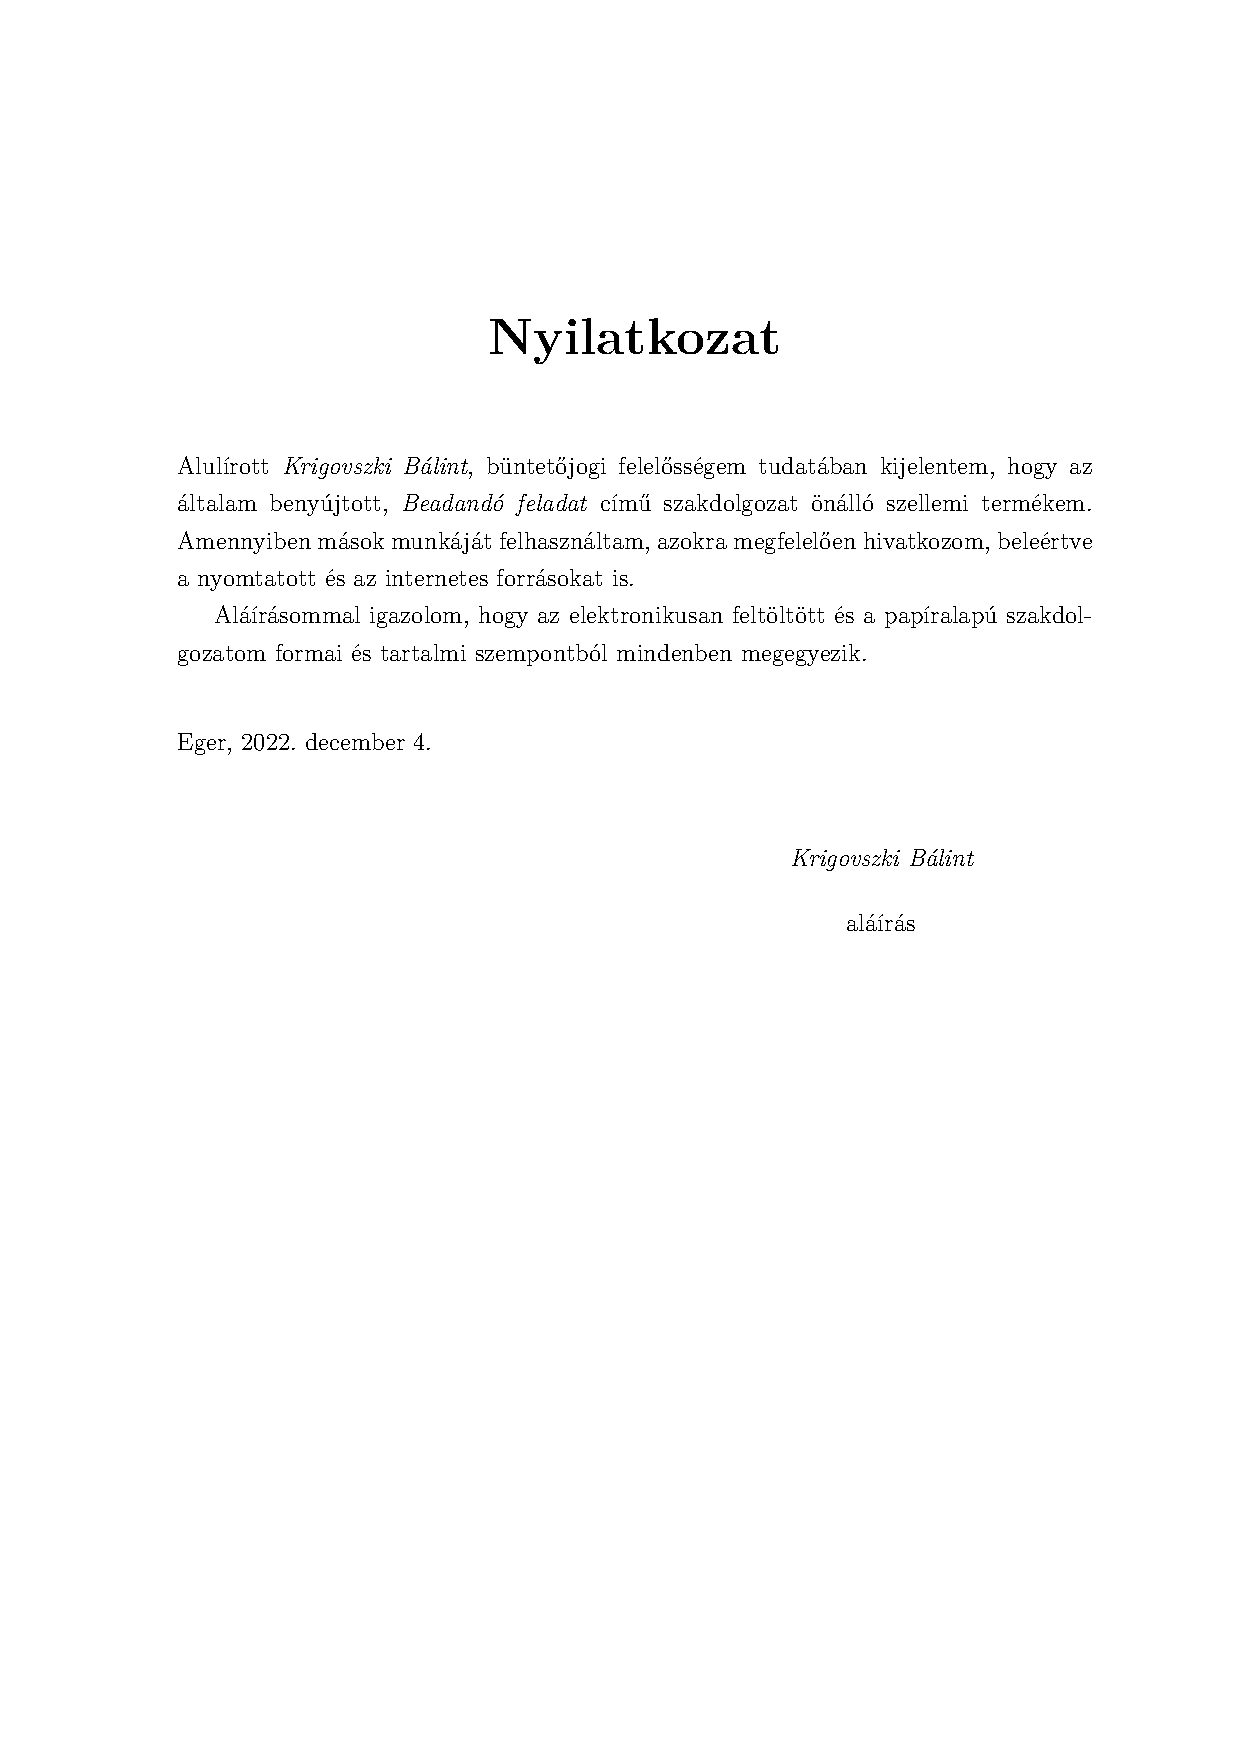
\includepdf{nyilatkozat.pdf}
\end{document}